%*****************************************
\chapter{Grundlagen}\label{ch:preliminaries}
%*****************************************

Dieses Kapitel wird nun zunächst die theoretischen Grundlagen betrachten, die zum Verständnis und zur Durchführung der geplanten methodischen Vorgehensweise notwendig sind.
Somit bekommen Fachfremde einen Einblick in die Themenbereiche der medizinischen Informatik, des Semantic Webs und des nutzerzentrierten Entwicklungsprozesses.

\section{Medizinische Informatik}\label{sec:mi}

Die Medizinische Informatik beschäftigt sich mit der systematischen Gewinnung, Verarbeitung, Speicherung und Bereitstellung von Daten im gesamten Gesundheitssystem. 
Die \ac{GMDS} lässt die Medizinische Informatik wie folgt definieren:

\begin{definition}
	Die Medizinische Informatik ist die Wissenschaft der systematischen Erschließung, Verwaltung, Aufbewahrung, Verarbeitung und Bereitstellung von Daten, Informationen und 			Wissen in der Medizin und im Gesundheitswesen.
\end{definition}

Das wichtigste Ziel der medizinischen Informatik ist die richtigen Informationen zur rechten Zeit am richtigen Ort in der richtigen Form dem richtigen Adressaten zur Verfügung zu stellen. 
Dadurch kann eine qualitative und effiziente Patientenversorgung sichergestellt werden. \citep[vgl.]{winter_health_2011}

\subsection{Daten, Information, Wissen}

Die drei Begriffe stehen hierarchisch in Beziehung zueinander.

\textbf{Daten} sind Symbole und Zeichen, die sich für die Kommunikation, Interpretation oder Verarbeitung durch Menschen oder Maschinen eignet.

\textbf{Informationen} sind in einem semantischen Kontext gesetzte Daten.
Informationen stellen Kenntnisse über Sachverhalte oder Personen dar.

\textbf{Wissen} beschreibt somit die gesammelte Information, die über die Begriffe einer bestimmten Domäne zur Verfügung stehen. 
Die Kenntnisse über diesen Sachverhalt ermöglichen es, fundierte Entscheidungen zu treffen und Probleme zu lösen.

\subsection{Krankenhausinformationssysteme}

Um den Begriff Krankenhausinformationssystem zu verstehen, werden erstmal die Begriffe System und Informationssystem betrachtet. \newline

Ein \textbf{System} ist eine Menge von Personen, Gegenstände, Ereignisse und deren Beziehungen zueinander. 
Ein System kann aus mehreren Subsystemen bestehen, die wiederum ein System darstellen. \citep[vgl.]{winter_health_2011} \newline

Ein \textbf{Informationssystem} ist der Teil einer Institution, das sich mit der Verwaltung und Speicherung von Daten, Informationen und Wissen beschäftigt.
Ein Informationssystem umfasst sowohl die gesamte Informationsverarbeitung als auch die dazugehörenden menschlichen oder technischen Akteure. \citep[vgl.]{winter_health_2011} \newline

Wenn man nun die zwei oben definierten Begriffe betrachtet, kann eine Krankenhausinfromationssystem wie folgt definiert werden:

\begin{definition}
	Ein Krankenhausinformationssystem ist das sozio-technische Subsystem eines Krankenhauses, das die gesamte Informationsverarbeitung sowie die zugehörigen menschlichen oder technischen Akteure in ihren jeweiligen Informationsverarbeitungsrollen umfasst. \citet{winter_health_2011}
\end{definition}

\subsection{Informationsmanagement in Krankenhäuser}



\section{Semantic Web}\label{sec:sw}

Das Semantic Web ist ein Netz von Daten, die so beschrieben und verknüpft sind, dass ein Kontext oder eine Semantik entsteht, die sich an definierte Grammatik- und Sprachkonstrukte halten. \citep[vgl.]{hebeler_semantic_2009}
Das Technologie-Stack worauf das Semantic Web basiert wird in der Abbildung \ref{fig:abb1} dargestellt.
Die Abbildung zeigt einerseits die logische Struktur des Semantic Webs, im Bild die Concepts\&Abstractions Seite des Technologie-Stacks und die andere Seite zeigt die eingeführten Technologien.
Das ist die Specifications\&Solutions Seite des Würfels.
In diesem Unterkapitel werden die grundlegenden Technologien des Semantic Webs vorgestellt, die relevant für die vorliegende Arbeit sind.

\begin{figure}[h]
	\centering
    	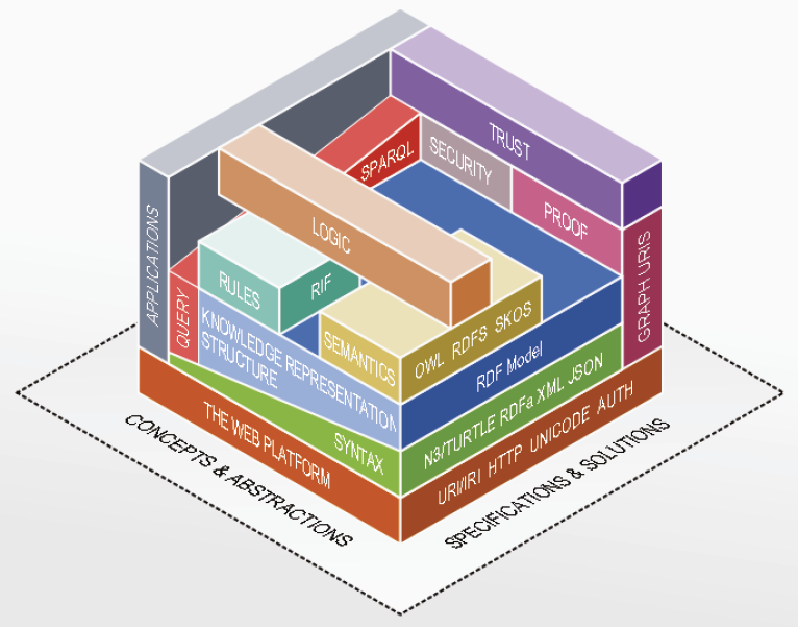
\includegraphics[width=0.65\textwidth]{Images/Linked_Data_Tech_Stack}
   	\caption{Semantic Web Technologie Stack}
   	\label{fig:abb1}
\end{figure}

\subsection{World-Wide Web}

Das \ac{WWW} ist eine Initiative, die verfügbare Technologien nutzt, um ein globales Informationsuniversum zu schaffen.
Grundlegend besteht das \ac{WWW} aus Inhalte, die primär an Menschen ausgerichtet sind.
Man wird von einer Seite zur anderen mittels \ac{URL}s weitergeleitet und der Nutzer muss in der Regel die Semantik selber ableiten.
Inhalte im \ac{WWW} werden beispielsweise mit Hilfe von HTML, CSS oder JavaScript formatiert.

Das Semantic Web soll als eine Erweiterung des WWW betrachtet werden.
Die Tabelle \ref{table:1} soll einen Vergleich zwischen dem \ac{WWW} und dem Semantic Web darstellen.

\begin{table}[h]
\begin{center}
\begin{tabular}{ | p{3 cm} | p{4 cm} | p{4 cm} | }
\hline
\textbf{Feature} & \textbf{WWW} & \textbf{Semantic Web} \\
\hline
grundlegende Komponente & unstrukturierte Inhalte & formale Statements \\ 
\hline
primäre Zielgruppe & Menschen & Applikationen \\ 
\hline
Links & geben den Ort an & geben den Ort und die Bedeutung an \\ 
\hline
vorwiegendes Vokabular & Formatierungsanweisungen & Semantik und Logik \\ 
\hline
Logik & informell/nicht standardisiert & Beschreibungslogik \\ 
\hline
\end{tabular}
\caption{Vergleich zwischen WWW und Semantic Web.}
\label{table:1}
\end{center}
\end{table}

\subsection{Ontologien}

Ontologien sind eine Form des Wissensmanagements und bilden den Kern aller Semantic Web Applikationen. 
Sie werden eingesetzt, um Wissen in einer strukturierten Weise zu organisieren.
Die Definition, die am häufigsten in der Literatur vorkommt, ist von \citet{gruber_translation_1993}:

\begin{definition}
  Eine Ontologie ist eine explizite Spezifikation einer Konzeptualisierung(Begriffsbildung).
\end{definition}

\noindent Aus Grubers Perspektive repräsentiert eine Ontologie das Wissen einer bestimmten Domain, wobei Objekte und deren Beziehungen mit Hilfe eines Vokabulars beschrieben werden. \citep[vgl.]{breitman_semantic_2007}

Im Bereich des Semantic Webs werden Ontologien als Graphen oder Netzwerkstrukturen betrachtet, die aus den folgenden Elementen bestehen:

\begin{itemize}
	\item eine Sammlung von Objekten (die Knoten des Graphs)
	\item eine Sammlung von Beziehungen, die die Objekte miteinander verknüpfen (Kanten des Graphs)
	\item eine Sammlung von Instanzen, die bestimmten Objekten zugeordnet sind (Daten die Objekten oder Relationen zugewiesen sind) \citep[vgl.]{davies_semantic_2006}
\end{itemize}

\subsection{RDF und RDF-Schema} 

\paragraph{RDF}

\ac{RDF} ist eine formale Sprache, die zur Beschreibung von strukturierten Informationen eingesetzt wird und ist somit eine der grundlegenden Bestandteile des Semantic Webs.
Das \ac{RDF}-Datenmodell ermöglicht den Austausch von Informationen im Web, ohne dass deren ursprüngliche Bedeutung verloren geht, und besitzt ein einfacher und flexibler Datenmodell. \citep[vgl.]{linkeddatavisualization}

Das Datenschema von \ac{RDF} basiert auf einer graph-orientierten Drastellung(?).
Die Knoten eines RDF-Graphen sind die Subjekte und die Objekte eines Statements.
Alle Ressourcen werden in RDF mit Hilfe von \ac{URI} bezeichnet.

\begin{itemize}
	\item graph-orientierte Datenschema
	\item eindeutige Namensgebung mittels URIs
	\item RDF-Snytax
	\item 
\end{itemize}

\paragraph{RDF-Schema} 

RDF- Schema bietet eine Möglichkeit Begriffe in Kategorien einzuteilen und über diese Kategorien Statements zu machen.
Somit können Onologien aufgebaut werden.
Durch RDF-Schema können dann zum Beispiel Klassen von Objekten definiert werden.
Für die Klassen können dann weiterhin Subklassen definiert werden und Eigenschaften können Werte- und Gültigkeitsbereiche zugeordnet werden. \citep[vgl.]{pellegrinix}

\begin{itemize}
	\item Klassen und Instanzen
	\item Unterklassen und Klassenhierarchien
	\item Propertys
	\item 
\end{itemize}

\subsection{OWL - Web Ontology Language}

RDF und RDFS sind für die Darstellung komplexer Zusammenhänge nicht ausreichend.

Erweiterung von RDF und RDF-Schema. 

OWL ist eine Ontologiesprache und basiert auf der Prädikatenlogik erster Stufe.

Wurde 2004 vom W3C als Ontologiepsrache standardisiert.

\begin{itemize}
	\item Klassen, Rollen und Individuen
	\item Arten von Beziehungen
	\item Propertys
	\item 
\end{itemize}

\subsection{SPARQL} 

Anfragesprache für RDF

\subsection{Linked (Open) Data} ??

\subsection{Visualisierung von Linked Data} ??

\section{Human-Computer Interaction}\label{sec:ux}

Die Art und Weise in der Menschen mit Computer interagieren hat sich über die Jahre stark verändert und steht in einer kontinuierlichen Entwicklung. 
Der Begriff  \ac{HCI}, in deutscher Sprache \ac{MMI} oder \ac{MCI}, wurde in den 1980er eingeführt.
Mit diesem Begriff wurde bestätigt, dass der Fokus nicht nur auf das Design der Benutzeroberfläche liegt, sondern alle Aspekte, die die Interaktion zwischen Nutzer und Computern betreffen, zu beachten sind. \citep[vgl.]{preece_human-computer_1995}
Ziel der Forschung im Rahmen von \ac{HCI} ist die stetige Verbesserung der Interaktion zwischen Menschen und Computern. \newline

\noindent Im Laufe der Jahre wurde keine einheitliche Definition für \ac{HCI} festgelegt.
Im Rahmen der \enquote{Encyclopedia of Database Systems} von \citet{dix_human-computer_2009} wurde \ac{HCI} wie folgt definiert:
\begin{definition}
  Human–Computer Interaction (HCI) is the study of the way in which computer technology influences human work and activities. 
  The term ‘‘computer technology’’ now-a-days includes most technology from obvious computers with screens and keyboards to mobile phones, household appliances, in-car navigation
  systems and even embedded sensors and actuators such as automatic lighting. 
  HCI has an associated design discipline, sometimes called Interaction Design or UserCentered Design, focused on how to design computer technology so that it is as easy and
  pleasant to use as possible.
\end{definition}

\noindent \citet{heimgartner_interkulturelles_2017} lässt \ac{HCI} zum Beispiel wie folgt definieren:

\begin{definition}
  Die Interaktion, bei der Information zwischen Benutzer und System via Benutzungsschnittstelle \ac{UI}) ausgetauscht wird, wird als \enquote{\ac{MMI}}  oder  \enquote{\ac{MCI}} 		 bezeichnet.
\end{definition}

\subsection{User Experience}

 \ac{UX} ist ein weitgreifender Ansatz, das \enquote{alle Aspekte der Erfahrungen eines Nutzers bei der Interaktion mit einem Produkt, Dienst, einer Umgebung oder Einrichtung} umfasst.
Ins Deutsche lässt sich der Begriff am besten als Nutzungserlebnis oder Nutzungserfahrung übersetzen. \citep[vgl.]{jacobsen_praxisbuch_2019}
Die Abbildung \ref{fig:abb2} zeigt, dass die \ac{UX} Aspekte vor, während und nach der Nutzung einer Anwendung betrachtet.
Aus der Abbildung kann beobachtet werden, dass Usability ein Teil der \ac{UX} ist.
Im nächsten Unterkapitel wird erläutert, was Usability ist und was man beachten muss, um eine gute Usability zu erreichen.

\begin{figure}[h]
	\centering
    	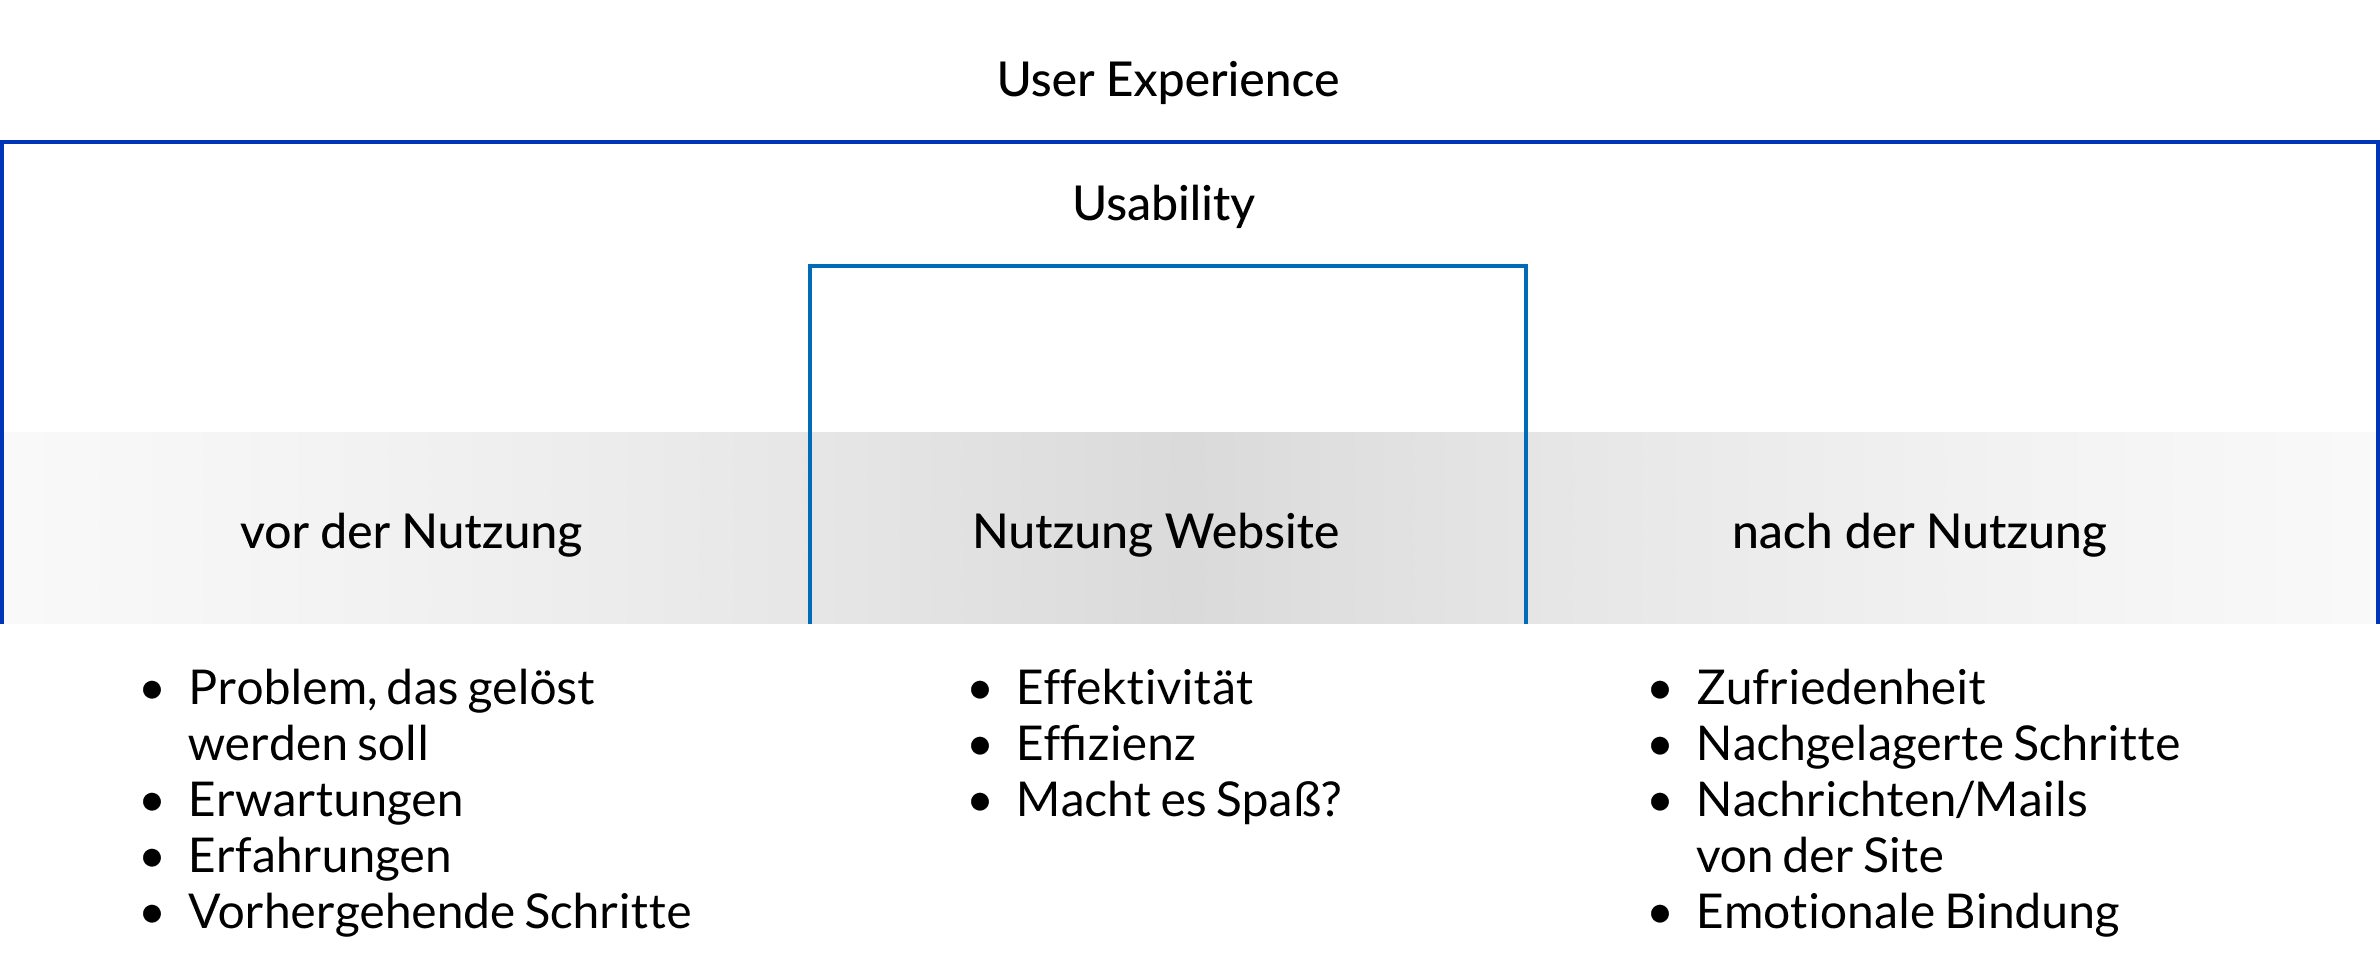
\includegraphics[width=0.99\textwidth]{Images/User_Experience.png}
   	\caption{Semantic Web Technologie Stack}
   	\label{fig:abb2}
\end{figure}

Nutzer sollen durch eine gute \ac{UX} positive Emotionen wie zum Beispiel Vorfreude, Spaß oder Zufriedenheit empfinden.
Die Erwartungen der Nutzer sollen erfüllt oder sogar übertroffen werden.
Faktoren, die die \ac{UX} positiv beeinflussen können, sind nicht nur die Usability sondern auch die Utility, die Ästhetik und die Markenwahrnehmung. \citep[vgl.]{weichert_quick_2021}

\subsection{Usability}

Die ISO-Norm 9241-11 bezeichnet Usability als \enquote{das Ausmaß, in dem ein Produkt, System oder Dienst durch bestimmte Benutzer in einem bestimmten Anwendungskontext genutzt werden kann, um bestimmte Ziele effektiv, effizient und zufriedenstellend zu erreichen}.

Daher besteht die Kernfrage der Usability daraus, ob der Nutzer seine Aufgaben und Ziele erfolgreich erreichen konnte.
Aus diesem Grund ist das Ziel von Usability, eine Anwendung so einfach wie möglich für den Benutzer zu gestalten. \citep[vgl.]{jacobsen_praxisbuch_2019}

Folgende Eigenschaften sollen laut der ISO-Norm 9241 erfüllt werden, um eine gute Usability zu gewährleisten :

\begin{itemize}
	\item \textbf{Der Aufgabe angemessen:} Die Anwendung soll die Erwartungen der Nutzer erfüllen. Nutzer sollen in der Lage sein ihre Ziele schnell zu erreichen.
	\item \textbf{Selbstbeschreibend:} Dem Nutzer soll deutlich gemacht werden, wie er sein Ziel erreicht. Die Navigation soll klar und verständlich gestaltet sein.
	\item \textbf{Steuerbar:} In diesem Fall, soll der Benutzer die Anwendung steuern und nicht umgekehrt. Zum Beispiel soll der Nutzer in der Lage sein zurück zur vorherigen Seiten kehren zu können.
	\item \textbf{Erwartungskonform:} Die Anwendung soll so gestaltet werden, dass Nutzer nicht überrascht werden. Etablierte Verhalten oder Elemente der Benutzeroberfläche sollen berücksichtigt werde. Zudem soll auch die Konsistenz innerhalb der Anwendung beachtet werden.
	\item \textbf{Fehlertolerant:} Falsche Benutzereingaben sollen betrachtet werden. Dabei muss dem Nutzer der Fehler signalisiert werden und eine schnelle Korrektur soll gewährleistet werden.
	\item \textbf{Individualisierbar:} Die Anwendung soll dem Nutzer die Möglichkeit geben, seine Angaben zu speichern und diese bei dem nächsten Besuch nicht erneut eingeben zu müssen.
	\item \textbf{Lernförderlich:} Die Anwendung soll den Benutzer dabei unterstützen, den Umgang schrittweise zu erlernen, beispielsweise durch Tastaturkürzel.
\end{itemize}

\subsection{User-Centered Design}

Das \ac{UCD} ist eine Methodik, die von Software-Entwickler und Designer im Bereich von Software Design angewendet wird. 
Die Methode hilft dabei Software zu entwickeln, die der Bedürfnisse der Nutzer entspricht. \cite[vgl.]{salinas_2020}

\begin{definition}

User-Centered Design bezeichnet ein Vorgehen, das durch die direkte Einbeziehung der Nutzer, frühe Visualisierung in From von Prototypen und ein iteratives Vorgehen sicherstellt, dass die Erwartungen der Nutzer erfüllt oder übertroffen werden und das Nutzungserlebnis positiv ausfällt. \citet{weichert_quick_2021}

\end{definition} 

Laut dem ISO 13407 Standard, besteht die Methodik aus den vier folgenden Schritte:

\begin{enumerate}
	\item Verstehen und Spezifizieren des Nutzungskontextes (Analyse)
	\item Spezifizierung der Benutzer- und Organisationsanforderungen (Konzeption)
	\item Entwurfslösungen erstellen (Design)
	\item Entwürfe anhand der Anforderungen zu bewerten (Evaluation)
\end{enumerate}
